% =========================================================
% Results / Preprint — arXiv style (VDM-aligned)
% Requires: arxiv.sty in the project (use Overleaf's arXiv template)
% =========================================================
\documentclass{article}

% ---- arXiv preprint look ----
\usepackage{arxiv}              % provided by the arXiv template
\usepackage[utf8]{inputenc}
\usepackage[T1]{fontenc}
\usepackage{lmodern}

% ---- math, figures, tables ----
\usepackage{amsmath, amssymb, amsthm, mathtools}
\usepackage{graphicx}
\usepackage{booktabs}
\usepackage{siunitx}
\sisetup{detect-all}
\usepackage{microtype}

% ---- refs & links (arXiv template uses natbib) ----
\usepackage{natbib}
\usepackage{doi}
\usepackage[hidelinks]{hyperref}

% ---- OPTIONAL: line numbers (comment out if not needed) ----
% \usepackage[modulo]{lineno}

% ---- Minimal gate + provenance helpers (no box styles) ----
\newenvironment{vdmgate}[2]{%
  \paragraph{Gate: #1} \emph{Threshold: #2.}%
  \par\noindent}{\medskip}
\newcommand{\provenance}[3]{\textbf{Commit:} \texttt{#1}\quad
  \textbf{Seed:} \texttt{#2}\quad
  \textbf{Artifacts:} \texttt{#3}}

% ---- Metadata (edit) ----
\title{RESULTS / PREPRINT TITLE}
\author{Justin K.\ Lietz\\
Neuroca, Inc.\\
\texttt{justin@neuroca.ai}}
\date{\today}

% Short header (optional)
\renewcommand{\headeright}{A PREPRINT}
\renewcommand{\undertitle}{}
\renewcommand{\shorttitle}{Results / Preprint}

\begin{document}
\maketitle
% \linenumbers

\begin{abstract}
One concise paragraph: scope, standard terminology (first), VDM label (parentheses),
primary gate(s) with thresholds, and where the evidence lives (figures/tables/artifacts).
\end{abstract}

\keywords{reaction–diffusion \and metriplectic \and reproducibility \and scaling}

% =========================================================
\section{Introduction}
State exactly what is claimed and not claimed. Give the evaluation question in one sentence.
Keep related work focused (2–4 citations) on the most relevant baselines.

% =========================================================
\section{Background}
\subsection*{Scope and larger theory}
Situate within a standard framework (e.g., gradient flows / Onsager; metriplectic structure) and why it fits.

\subsection*{Core equations used later}
List only the equations you actually use (invariants, discretizations, error models) with symbol definitions and units.

\subsection*{Map to gates}
Tie each property to a concrete metric/threshold you’ll test in Results.

% =========================================================
\section{Methods}
\subsection*{Variables}
Independent/dependent variables, units, ranges, estimator/uncertainty.

\subsection*{Equipment / Software Stack}
Hardware, ROCm version, library versions, precision/modes.

\subsection*{Procedure}
Steps sufficient for replication; third-person, past tense.

\subsection*{Provenance}
\provenance{<commit-hash>}{<seed>}{<https://…/artifacts/>}

% =========================================================
\section{Results}
Report processed data with uncertainties; one claim per figure. Captions carry numbers
(slope, $R^2$, RMSE) \emph{and} paired CSV/JSON filenames plus seed/commit.

\begin{figure}[t]
  \centering
  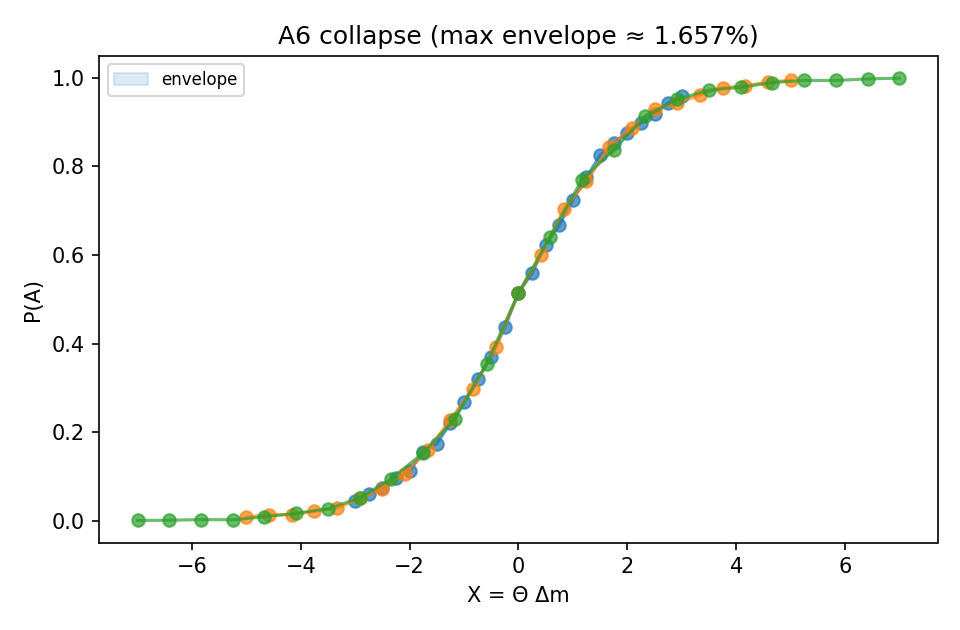
\includegraphics[width=0.8\linewidth]{figures/example-result}
  \caption{Front-speed vs.\ theory; slope $0.98$, $R^2=0.995$.
  Paired artifacts: \texttt{front\_speed.csv}, \texttt{front\_speed.json};
  seed \texttt{<seed>}, commit \texttt{<commit>}.}
  \label{fig:frontspeed}
\end{figure}

\begin{table}[t]
  \centering
  \caption{Summary metrics with uncertainties.}
  \label{tab:summary}
  \begin{tabular}{@{}lrrr@{}}
  \toprule
  Metric & Mean & Std & N \\
  \midrule
  <metric A> & <..> & <..> & <..> \\
  \bottomrule
  \end{tabular}
\end{table}

% =========================================================
\section{Gates and Contradictions}
\begin{vdmgate}{Front-speed accuracy}{relative error $\le 5\%$}
Measured: $3.2\%$ on $n=8$ seeds. \textbf{PASS}. Artifacts: \texttt{front\_speed.csv/json}.
\end{vdmgate}

\begin{vdmgate}{Dispersion RMSE}{$\mathrm{RMSE}\le 2\times 10^{-3}$}
Measured: $2.4\times10^{-3}$. \textbf{FAIL}. See contradiction report:
\texttt{dispersion\_fail.json}.
\end{vdmgate}

% =========================================================
\section{Discussion}
Interpret the patterns with explicit pointers to Figs./Tables. Bound claims by artifacts and note limits.

% =========================================================
\section{Conclusions}
Concise restatement, limits, and next testable gate(s).

% =========================================================
\section{Runtime and Scaling}
Report P50/P95/P99 step time, jitter, active-site fraction, and log–log slope $\beta$ with CIs.

\begin{table}[t]
  \centering
  \caption{Runtime and scaling disclosure.}
  \label{tab:runtime}
  \begin{tabular}{@{}lrrrr@{}}
  \toprule
  Metric & P50 & P95 & P99 & Notes \\
  \midrule
  Step time (ms) &  &  &  & \\
  Active-site fraction &  &  &  & \\
  Slope $\beta$ (log–log) &  &  &  & CI: [\,\,] \\
  \bottomrule
  \end{tabular}
\end{table}

% =========================================================
\bibliographystyle{unsrtnat}  % arXiv template default-ish (numeric, unsorted by appearance)
\bibliography{references}     % create references.bib or inline with thebibliography

\end{document}
